\documentclass{sbc2019}%

\usepackage{graphicx}
\usepackage[utf8]{inputenc}
%\usepackage[brazil]{babel}
\usepackage[misc,geometry]{ifsym} 
%\usepackage{fontspec}       % Requer XeLaTeX/LuaLaTeX - removido para compatibilidade com PdfLaTeX
\usepackage{fontawesome5}    % Substituto do fontawesome compatível com PdfLaTeX
%\usepackage{academicons}   % Requer fontspec - removido para compatibilidade com PdfLaTeX
\newcommand{\aiOrcid}{\textsuperscript{\textbf{iD}}} % Fallback para o ícone ORCID
\usepackage{multirow}
\usepackage{array}
\usepackage[version=4]{mhchem}
\usepackage{color}
\usepackage{hyperref}
\usepackage{aas_macros}
\usepackage[bottom]{footmisc}

\usepackage{booktabs}
\usepackage{makecell}
\usepackage{comment}

% COLOR
\usepackage{xcolor,color}
\newcommand{\todo}[1]{\textcolor{red}{#1}} 
\newcommand{\blue}[1]{\textcolor{blue}{#1}} 
\newcommand{\new}[1]{\textcolor{orange}{#1}}
\newcommand{\joey}[1]{\textcolor{darkgreen}{#1}} 

\definecolor{orcidlogo}{rgb}{0.37,0.48,0.13}
\definecolor{unilogo}{rgb}{0.16, 0.26, 0.58}
\definecolor{maillogo}{rgb}{0.58, 0.16, 0.26}
\definecolor{darkblue}{rgb}{0.0,0.0,0.0}
\definecolor{darkgreen}{rgb}{0.0, 0.5, 0.0}
\definecolor{myred}{rgb}{0.75, 0.1, 0.1}

\hypersetup{colorlinks,breaklinks,
            linkcolor=darkblue,urlcolor=darkblue,
            anchorcolor=darkblue,citecolor=darkblue}
%\hypersetup{colorlinks,citecolor=blue,linkcolor=blue,urlcolor=blue}

%%%%%%% IMPORTANT: We disable hyperlinks by default with this line, to avoid the error "\pdfendlink ended up in different nesting level" while writing.
%\hypersetup{draft}

\jid{JSERD}
\jtitle{Journal of Software Engineering Research and Development, 2026, 6:1, }
\doi{10.5753/jserd.2026.xxx}
\copyrightstatement{This work is licensed under a Creative Commons Attribution 4.0 International License.}
\jyear{2026}



\title[Client-Side vs Server-Side Rendering: Impacts on Performance and User Experience in Web Applications]


%% Please note that the command \and is not supported in \author.

\author[Clapton et al. 2026]{
\affil{\href{}{\textcolor{orcidlogo}{\aiOrcid}}~\textbf{Joey Clapton}~~\textcolor{unilogo}{\faUniversity}~\textbf{Pontifical Catholic University of Minas Gerais (PUC Minas)~~}\href{mailto:joeyclapton42@gmail.com}{\textcolor{maillogo}{\faEnvelope}}~\textbf{\textit{joeyclapton42@gmail.com}}}

\affil{\href{https://orcid.org/0009-0001-7655-9578}{\textcolor{orcidlogo}{\aiOrcid}}~\textbf{João Pedro Oliveira Batisteli}~~\textcolor{unilogo}{\faUniversity}~\textbf{Pontifical Catholic University of Minas Gerais (PUC Minas)~~}\href{mailto:joao.batisteli@sga.pucminas.br}{\textcolor{maillogo}{\faEnvelope}}~\textbf{\textit{joao.batisteli@sga.pucminas.br}}}

\affil{\href{https://orcid.org/0000-0002-6193-3205}{\textcolor{orcidlogo}{\aiOrcid}}~\textbf{Hugo Bastos de Paula}~~\textcolor{unilogo}{\faUniversity}~\textbf{Pontifical Catholic University of Minas Gerais (PUC Minas)~~}\href{mailto:hugo@pucminas.br}{\textcolor{maillogo}{\faEnvelope}}~\textbf{\textit{hugo@pucminas.br}}}

\affil{\href{https://orcid.org/0000-0002-0155-7631}{\textcolor{orcidlogo}{\aiOrcid}}~\textbf{Danilo Boechat Seufitelli}~~\textcolor{unilogo}{\faUniversity}~\textbf{Federal Center for Technological Education of Minas Gerais (CEFET-MG)~~}\href{mailto:danilobs@cefetmg.br}{\textcolor{maillogo}{\faEnvelope}}~\textbf{\textit{danilobs@cefetmg.br}}}

\affil{\href{https://orcid.org/0009-0008-4235-409X}{\textcolor{orcidlogo}{\aiOrcid}}~\textbf{Cleiton Tavares}~~\textcolor{unilogo}{\faUniversity}~\textbf{Pontifical Catholic University of Minas Gerais (PUC Minas)~~}\href{mailto:cleitontavares@pucminas.br}{\textcolor{maillogo}{\faEnvelope}}~\textbf{\textit{cleitontavares@pucminas.br}}}
}

%%%%%%% You may comment or delete the line above to make hyperlinks in your paper active. If you then encounter a strange "\pdfendlink ended up in different nesting level than \pdfstartlink", don't worry! Uncomment the line again, and see https://www.overleaf.com/help/246 for further information.

\begin{document}

\begin{frontmatter}
\maketitle

\begin{abstract}
\textbf{Abstract}

The increasing complexity of web applications necessitates careful selection of rendering strategies to ensure optimal performance and user experience. This study presents a comparative analysis of Client-Side Rendering (CSR) and Server-Side Rendering (SSR) techniques, evaluating their impact on web application quality based on Google's Core Web Vitals metrics (CWV).  In this work, photo gallery web applications were implemented using both rendering approaches to allow a homogeneous environment for comparable results.
Through controlled experiments across five data sizes (ranging from 498 kB to 26 MB), measurements were taken for key performance indicators, including First Contentful Paint (FCP), Speed Index (SI), Time to Interactive (TTI), Largest Contentful Paint (LCP), and JavaScript Heap Used. Statistical analysis using the Kruskal-Wallis test revealed significant performance differences ($p \leq$ 0.05) in all metrics. Results show that SSR achieves superior performance in TTI (mean reduction of 62.3\%) and LCP (mean reduction of 58.7\%), particularly under increased data loads, while CSR exhibits better FCP and SI performance for smaller datasets. The results suggest that the choice between CSR and SSR should consider the application's specific objectives and usage environment. 
These findings contribute to evidence-based decision-making frameworks for web application architecture, supporting software quality engineering practices in modern development environments.
\end{abstract}

\begin{keywords}
Proceedings, Template, BCS, Content Repository, Indexing
\end{keywords}

%\begin{license}
%Published under the Creative Commons Attribution 4.0 International Public License (CC BY 4.0)
%\end{license}


\end{frontmatter}


\input{src/01.Introduction}

% \begin{table}[!ht]
% \caption{This is an example of table caption.}
% \centering
% \begin{tabular}{@{}cc@{}}
% \hline\hline
% Dimension & Classification accuracy \\
% \hline%
%  1  & 0.6232 \\
%  2  & 0.9635 \\ 
%  3  & 0.9724 \\ 
%  4  & 0.9690 \\ 
%  5  & 0.9840 \\ 
%  6  & 0.9842 \\ 
%  7  & 0.9873 \\ 
%  8  & 0.9884 \\
%  9  & 0.9873 \\ 
%  10 & 0.9898 \\ 
%  11 & 0.9914 \\
% \hline\hline
% \end{tabular}
% \label{tab1}
% \end{table}

 
\section{Background}\label{sec:background}

This section presents the key concepts related to the study. Section \ref{sec:ssr} describes the SSR method. Section \ref{sec:csr} discusses CSR method. Section \ref{sec:performance_aspects} addresses software performance aspects, and Section \ref{sec:quality_indicators} covers quality indicators in web applications based on  Core Web Vitals (CWV) metrics.

%Fiz pequenas mudanças.
\subsection{Server-Side Rendering (SSR)}
\label{sec:ssr}

Server-Side Rendering (SSR) is a web application development methodology in which pages are rendered on the server and sent to the browser \cite{clientServerSide:2020}. When a request is made, the server processes it and returns the page already rendered in HTML to the user's browser.

% In applications that use SSR rendering is handled on the server side, allowing the page to be fully loaded when accessed by the user \citet{clientServerSide:2020}. This results in a faster user experience, especially on low-performance devices, since the server handles the more computationally expensive tasks. Additionally, SSR offers advantages in terms of search engine rankings, as it allows search engines to more easily index page content.

In applications that use SSR, the rendering process is handled on the server, enabling the page to be fully loaded when accessed by the user \citet{clientServerSide:2020}. This approach improves the user experience, particularly on low-performance devices, as the server performs the more computationally intensive tasks. Moreover, SSR provides advantages in search engine optimization (SEO), as it facilitates the indexing of page content by search engines.

\subsection{Client-Side Rendering (CSR)}
\label{sec:csr}

Client-Side Rendering is a web page rendering mechanism in which the rendering process takes place in the user's browser \cite{clientServerSide:2020}. The server sends a basic HTML structure with JavaScript responsible for dynamically rendering the content on the client side.

% According to \citet{clientServerSide:2020} CSR allows for more dynamic and interactive applications, as rendering logic and manipulation of the Document Object Model (DOM) occur directly in the user's browser. This can lead to a smoother user experience, especially in highly interactive applications such as Single Page Applications (SPAs), where navigation between pages does not require a full page reload.

CSR enables the development of more dynamic and interactive applications, as both the rendering logic and Document Object Model (DOM) manipulation are executed directly within the user's browser \cite{clientServerSide:2020}. This approach can deliver a smoother and more responsive user experience, particularly in highly interactive scenarios such as Single Page Applications (SPAs), where navigation between views occurs without the need for full page reloads.

\subsection{Software Performance Aspects}
\label{sec:performance_aspects}

A software performance aspect refers to a non-functional characteristic that describes the operational efficiency of a software system under various execution conditions~\cite{performanceAspects}. These aspects are essential to ensure that the software meets the expected quality and efficiency demanded by users. Key performance metrics include response time, which measures how long the system takes to respond to a request, and resource usage, which evaluates the memory and CPU consumption during application operations.

Performance aspects are critical to user experience, user retention, and the overall success of a web application. Pages that load slowly or respond poorly can frustrate users and cause them to abandon the site. Good performance is also important for Search Engine Optimization (SEO), as search engines tend to favor fast-loading websites~\cite{clientServerSide:2020}. As a result, optimizing these performance aspects has become a crucial part of developing and maintaining websites, requiring an integrated approach that considers both operational efficiency and end-user experience~\cite{pageExp:2022}.

\subsection{Quality Indicators in Web Applications Based on Core Web Vitals Metrics}
\label{sec:quality_indicators}

CWV is a set of performance metrics introduced by Google\footnote{\url{https://developers.google.com/web/tools/lighthouse}} to help optimize and evaluate the user experience of web pages, guiding improvements in the user experience. The CWV includes:

\textbf{Largest Contentful Paint (LCP)}: measures the loading time of the largest content element visible to the user.

\textbf{First Input Delay (FID)}: measures the time from the user's first interaction to the browser's response.

\textbf{Cumulative Layout Shift (CLS)}: evaluates layout shifts during page loading.

\textbf{First Contentful Paint (FCP)}: measures how quickly content is rendered to the screen, ensuring users see something useful sooner.

\textbf{Speed Index (SI)}: measures how quickly visible content is displayed during page loading, influencing user experience and search engine ranking.

\textbf{Time to Interactive (TTI)}: evaluates page usability. A faster TTI means users can interact with the page sooner.

\section{Related Work}\label{sec:related_work}

The related works presented in this section discuss studies connected to the context of quality indicators in web applications based on Core Web Vitals (CWV) metrics, evaluation and comparison of performance aspects, and identification and comparison of computational costs in web applications.

\citet{parsingJson:2019} present  \textit{simdjson} tool, a high-performance solution for processing large volumes of data in JSON. The study emphasizes that, with the growing exchange of structured data in web applications, the performance of traditional parsers has become a bottleneck. \textit{Simdjson} outperforms reference analyzers such as RapidJSON by employing optimized techniques for detecting JSON structures. Thus, the study conceptually contributes to the present study by highlighting how the interpretation and manipulation of JSON data can directly impact overall application performance, particularly in contexts where different rendering strategies are compared.

\citet{webPerformanceOptimize:2023} analyzed an industrial case study in an agricultural technology company aiming to improve the performance of a large-scale web dashboard. The authors developed a performance engineering plan using a benchmarking tool based on Google Lighthouse to assess the impact on web performance metrics. The results demonstrated a significantly faster browsing experience, with pages loading 98.37\% faster on desktop devices and 97.56\% faster on mobile. Content rendering also became more efficient, with improvements of 48.25\% and 19.85\% in rendering speed on desktop and mobile devices, respectively. This study is relevant to the current research as it provides data on the impact of different interventions affecting performance metrics using Google Lighthouse. However, there remains a gap for analyzing performance during data transactions between JSON and HTML formats using the same tool.

\citet{webAutoscaling:2022} explored mechanisms to ensure the resilience and performance of web applications under high-demand scenarios and potential failures. The study investigated different scaling approaches for applications and databases, such as horizontal and vertical scaling, database replication, and sharding, focusing on achieving fault tolerance and autoscaling capabilities. The authors emphasize the importance of making applications stateless by using external solutions for session storage and user files to facilitate horizontal scaling. The study concludes that to build a fault-tolerant web application, scalability is essential, and autoscaling can significantly reduce manual configuration time and improve responsiveness to traffic spikes. The research offers insights into how different scaling strategies can influence the performance and resilience of web applications, critical aspects also considered in the comparison between CSR and SSR.

\citet{clientServerSide:2020} investigated the performance of web applications built using CSR and SSR rendering techniques. The study developed a web application named Show Up using both approaches and compared their performance based on FCP, Speed Index, TTI, and FMP metrics. The results showed that SSR rendering outperformed CSR across all evaluated metrics, delivering a faster and smoother user experience. In addition, SSR scored higher on Google audit metrics for performance, accessibility, and best practices. The authors provide a discussion on different rendering strategies and their implications for application performance. This enables further investigation into other contributing factors, such as the impact of JSON and HTML data formats on user experience and web application efficiency, analyzed in the present study.

\section{Metodology}\label{sec:materiais}

This study conducts a quantitative experimental research by investigating and comparing the performance, computational cost, and CWV metrics analysis between SSR and CSR for data presentation in web applications. The following subsections describe the development environment, which consists of a web application. Subsequently, the materials and methods used in the experiment are detailed, including performance measurement tools, computational cost metrics, and the different data sizes analyzed.

\subsection{Study Steps}

The study was divided into three steps, which are described as follows.

% This section presents the three main stages of development for this study.

In the \textit{first step}, the data were defined and created in JSON format. The datasets were generated in five different sizes: 498 kB, 2 MB, 7.9 MB, 16.8 MB, and 26 MB. Each dataset was composed by combining 13 different images, resulting in: 370 images (498 kB), 1,500 images (2 MB), 6,000 images (7.9 MB), 12,000 images (16.8 MB), and 19,000 images (26 MB).
These sizes were selected based on the study by~\citet{jsonXmlCaseStudy:2009}, which analyzed the performance of data interchange formats in various scenarios. For the experiment, a data structure was designed to simulate a photo gallery system using JSON (Figure~\ref{fig:jsonStructure}). The choice of this data structure aims to represent a real-world use case where user information is frequently exchanged between systems.

\begin{figure}[tb]
\centering
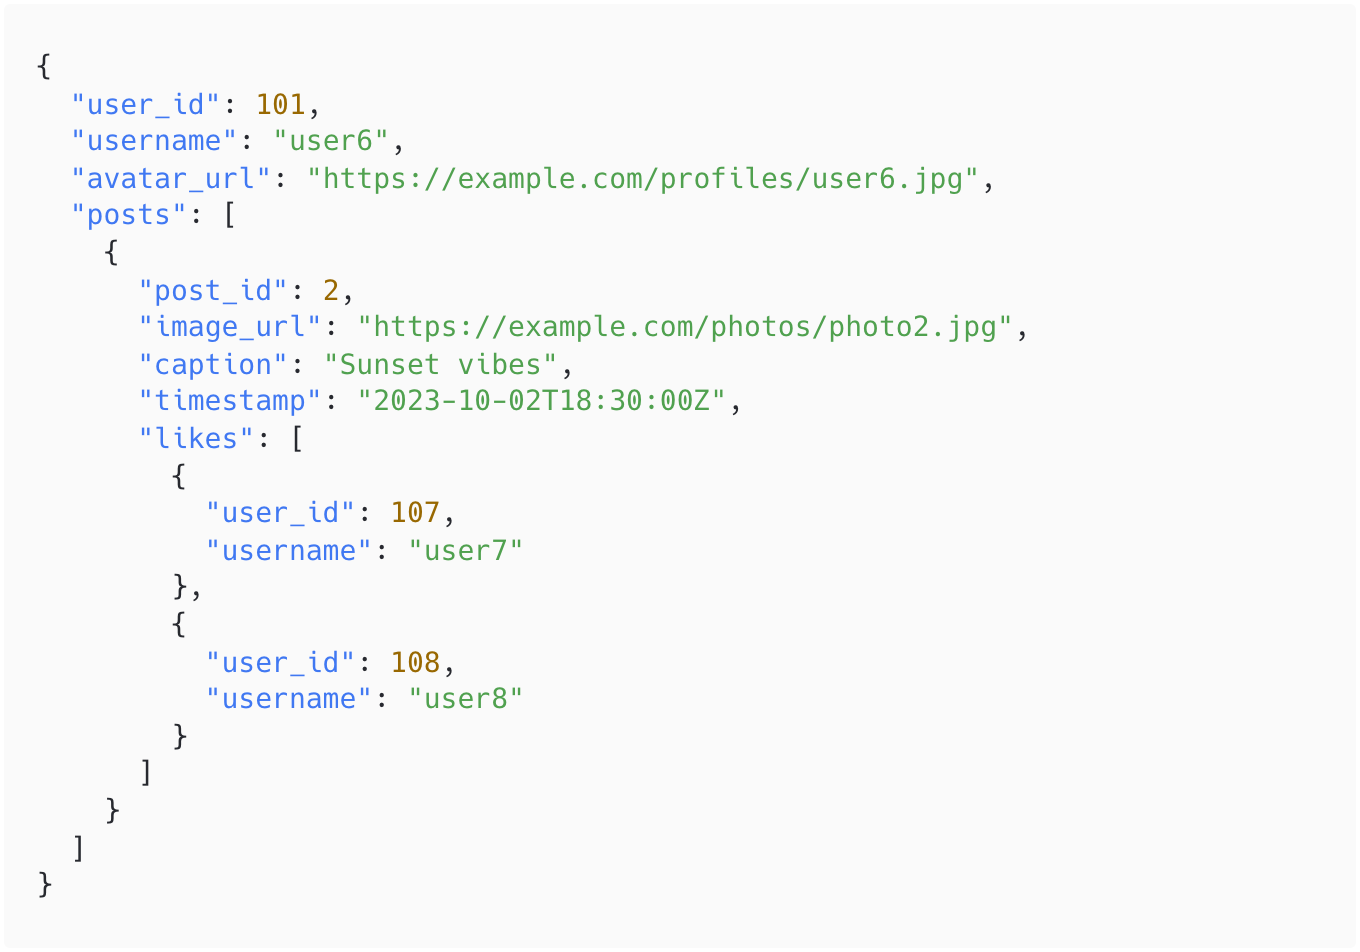
\includegraphics[width=.45\textwidth]{img/03-json-structure.png}
\caption{JSON data structure used in the application}
\label{fig:jsonStructure}
\end{figure}

Furthermore, a back-end application was developed using the NodeJS platform. An Application Programming Interface (API) was created to handle two parameters: data size and rendering type (SSR or CSR). Based on these parameters, the API returns either the HTML rendered from the JSON or the raw JSON itself to the client. The data is stored locally.

The \textit{second step} %involved developing a front-end application in JavaScript. This application (Figure~\ref{fig:exampleFig2}) allows users to select both the size and format of the data to be requested. It then sends the request to the back-end and displays the response, which may either be the fully rendered HTML from the server or the raw JSON used to dynamically build the web page.
consisted of developing a front-end application in JavaScript. As illustrated in Figure~\ref{fig:exampleFig2}, this application enables users to select both the size and format of the data to be requested. Once the request is sent to the back-end, the application displays the response, which can either be the fully rendered HTML returned by the server or the raw JSON used to dynamically build the web page.

\begin{figure}[tb]
\centering
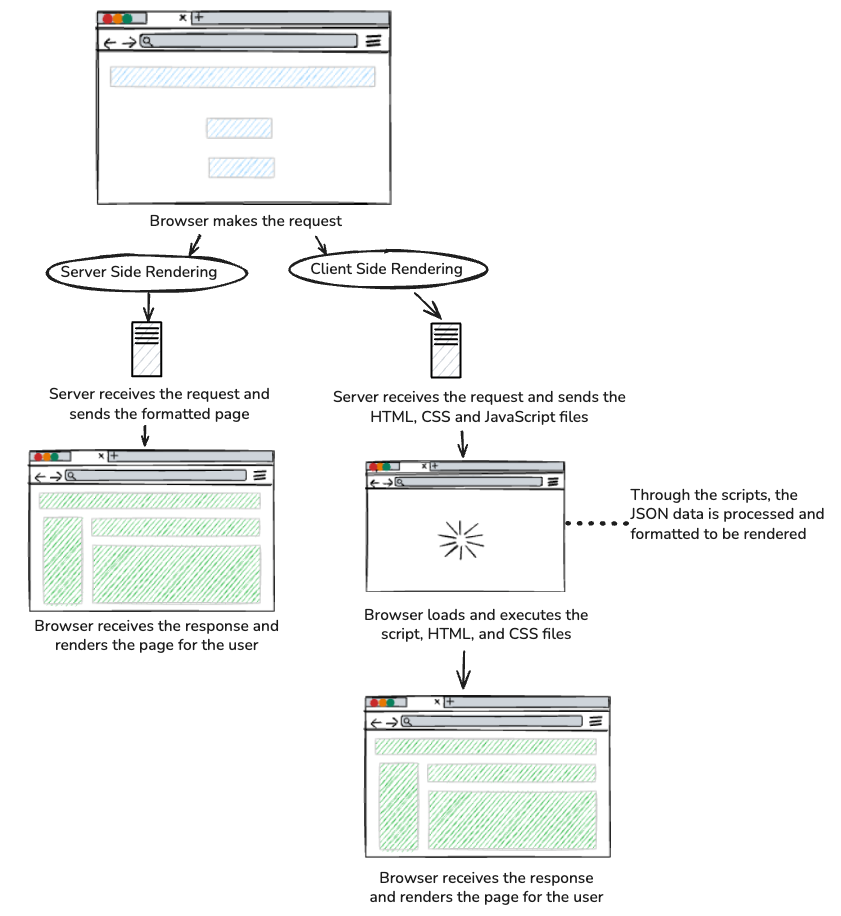
\includegraphics[width=.5\textwidth]{img/04-csr-ssr.png}
\caption{Application operation flow}
\label{fig:exampleFig2}
\end{figure}

Subsequently, a JavaScript script was developed to evaluate application performance. %The script uses the Lighthouse library to automatically calculate key performance metrics. Additionally, the \texttt{chrome-launcher} library was employed to launch a clean instance of the Chrome browser for performance testing. The Puppeteer tool\footnote{\url{https://pptr.dev/}} was also used to collect profiling metrics and computational cost data. Each configuration (JSON and HTML) was tested 10 times, and the average execution time was computed to yield more accurate and representative results. The following metrics, were analyzed in this study:
Leveraging the Lighthouse library, the script automatically computes key performance metrics. To ensure consistent testing conditions, the \texttt{chrome-launcher} library was used to start a clean instance of the Chrome browser. In addition, the Puppeteer tool\footnote{\url{https://pptr.dev/}} was used to collect profiling data and computational cost metrics. Each configuration (JSON and HTML) was tested 10 times, with the average execution time calculated to provide more accurate and representative results. The following metrics were analyzed in this study:

%%=============================
% Pra deixar o texto auto-contido, eu add uma breve explicação. Caso tenha algo errado, favor verificar Joey
% Na real percebi que ja tem explicação delas, exceto a última.
\begin{enumerate}
    \item \textbf{First Contentful Paint}%: Measures the time until the first piece of content (e.g. text or image) renders on the screen.
    \item \textbf{Speed Index}%: Measures how quickly the content within the visible area (viewport) is visually populated.
    \item \textbf{Time to Interactive}%: Measures the time for a page to become fully responsive to user interactions.
    \item \textbf{Largest Contentful Paint}%: Measures the render time of the largest content element (image or text block) within the visible area.
    \item \textbf{\textit{JS Heap} Size}%: Measures memory usage by JavaScript, indicating the application's computational cost.
\end{enumerate}

In the \textit{third step}, the Kruskal-Wallis statistical test\footnote{Kruskal-Wallis is a non-parametric test used for comparing three or more independent samples.} was applied to validate the significance of the results across the different data formats tested. Core Web Vitals metrics were evaluated to understand the impact of data formats on user experience.

\joey{Additionally, we adopted Cliff's Delta ($\delta$) as an effect size measure to quantify the magnitude of the observed differences between the experimental groups. This non-parametric statistic calculates the probability that a randomly selected observation from one group is larger than an observation from another group \cite{Cliff1993}. This method is suitable for non-normal data distributions, as confirmed by the Shapiro-Wilk tests conducted in this study. The $\delta$ values range from $-1$ to $+1$. We interpreted these values according to the thresholds proposed by \citet{Romano2006}: $|\delta| < 0.147$ (\textit{negligible}), $0.147 \leq |\delta| < 0.33$ (\textit{small}), $0.33 \leq |\delta| < 0.474$ (\textit{medium}), and $|\delta| \geq 0.474$ (\textit{large}).} 

\joey{We justified the use of this measure because the $p$-value alone does not indicate the practical magnitude of the observed differences. Solely relying on $p$-values can lead to overestimated interpretations in experiments with controlled conditions \cite{Kitchenham2017, Torkar2022}. We calculated 95\% confidence intervals using the bootstrap method with 10,000 resamples \cite{efron:1994}. For pairwise comparisons between groups, we applied Dunn's post-hoc test with Holm's correction to adjust for multiple comparisons \cite{Kitchenham2024}.
}

\begin{comment}
\joey{Adicionalmente, o Cliff's Delta ($\delta$) foi adotado como medida de tamanho de efeito (\textit{effect size}) para quantificar a magnitude das diferenças observadas entre os grupos experimentais. Trata-se de uma estatística não paramétrica que calcula a probabilidade de que uma observação selecionada aleatoriamente de um grupo seja maior do que uma observação do outro grupo \cite{Cliff1993}, sendo adequada para dados com distribuição não normal, conforme confirmado pelos testes de Shapiro-Wilk realizados neste estudo. Os valores de $\delta$ variam de $-1$ a $+1$ e foram interpretados segundo os limiares propostos por \citet{Romano2006}: $|\delta| < 0{,}147$ (\textit{negligible}), $0{,}147 \leq |\delta| < 0{,}33$ (\textit{small}), $0{,}33 \leq |\delta| < 0{,}474$ (\textit{medium}) e $|\delta| \geq 0{,}474$ (\textit{large}). A adoção dessa medida se justifica pelo fato de que o $p$-value, isoladamente, não informa a magnitude prática das diferenças observadas, podendo conduzir a interpretações superestimadas em experimentos com condições controladas \cite{Kitchenham2017, Torkar2022}. Intervalos de confiança de 95\% foram calculados por meio do método \textit{bootstrap} com 10.000 reamostragens \cite{efron:1994}. Para as comparações par a par entre os grupos, foi aplicado o teste post-hoc de Dunn com correção de Holm para ajuste de múltiplas comparações \cite{Kitchenham2024}.}

\end{comment}

\subsection{Photo Application}
Two photo gallery applications were developed: one focused on server-side rendering, and the other on client-side rendering, along with a selection page where the user can choose which rendering method will be displayed. Both applications were built using the same HTML structure, the same CSS styles, and without inserting any scripts, in order to prevent side effects on test results. Figure~\ref{fig:jsonStructure1} shows the initial selection page, while Figure~\ref{fig:jsonStructure2} shows the application running with client-side rendering using the smallest data size.

% \begin{figure}[h]
% \centering
% \begin{minipage}{0.47\textwidth}
%     \centering
%     
\includegraphics[width=\textwidth]{img/app02.png}
%     \caption{Data size and rendering type selection}
%     \label{fig:jsonStructure1}
% \end{minipage}\hfill
% \begin{minipage}{0.47\textwidth}
%     \centering
%     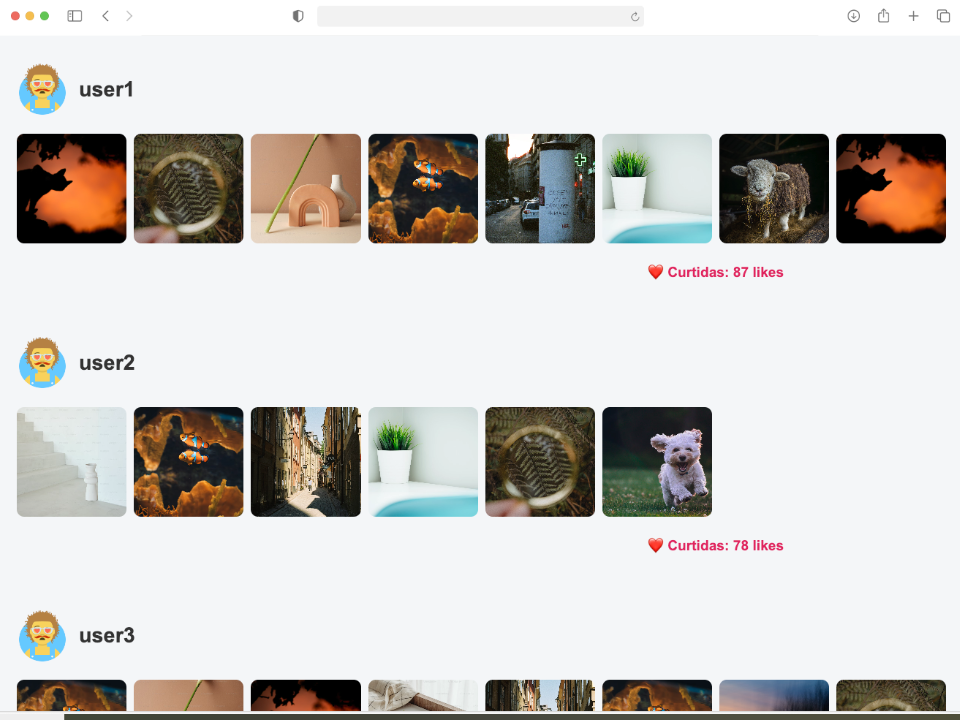
\includegraphics[width=\textwidth]{img/app-client.png}
%     \caption{Application using extra small data and CSR rendering}
%     \label{fig:jsonStructure2}
% \end{minipage}
% \end{figure}




\begin{figure}[tb]
\centering
    
\includegraphics[width=.45\textwidth]{img/app02.png}
    \caption{Data size and rendering type selection}
    \label{fig:jsonStructure1}
\end{figure}

\begin{figure}[tb]
\centering
    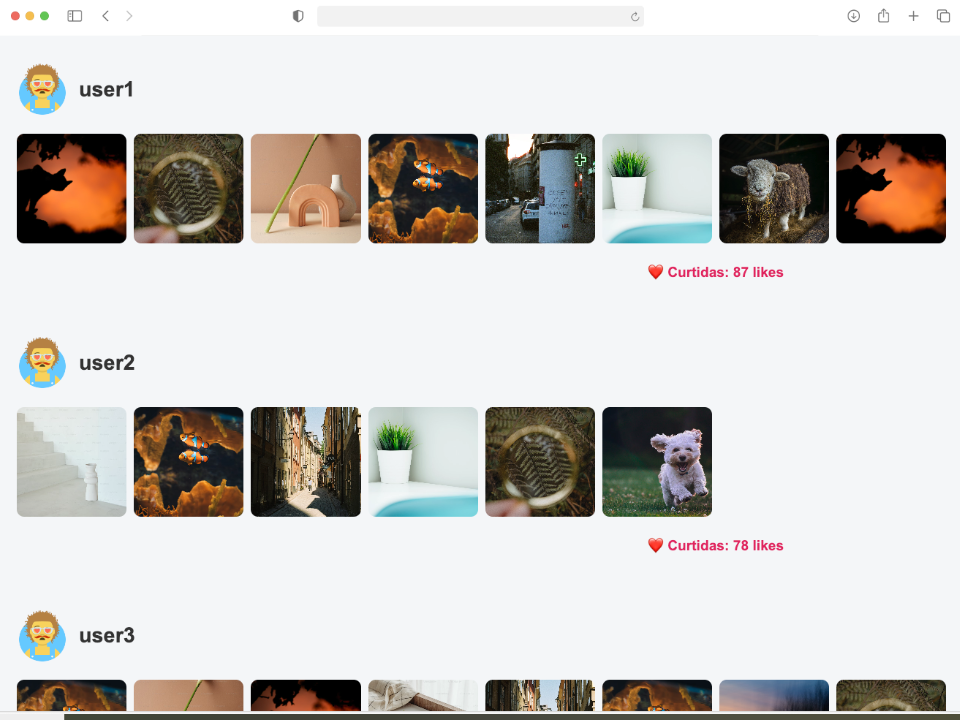
\includegraphics[width=.45\textwidth]{img/app-client.png}
    \caption{Application using extra small data and CSR}
    \label{fig:jsonStructure2}
\end{figure}

\subsection{\texorpdfstring{\textcolor{darkgreen}{Técnicas de Otimização de Desempenho}}{Técnicas de Otimização de Desempenho}}
\label{sec:optimization_techniques}

\textcolor{darkgreen}{Esta subseção descreve as técnicas de otimização de desempenho incorporadas ao estudo com o objetivo de investigar seus efeitos sobre as métricas de qualidade da aplicação. As técnicas adotadas foram a minificação dos dados JSON e a compressão por meio do algoritmo gzip. A inclusão dessas técnicas se justifica pela relevância prática que representam no desenvolvimento web, sendo amplamente utilizadas em ambientes de produção para reduzir o volume de dados trafegados na rede e, consequentemente, diminuir o tempo de carregamento das páginas \cite{sikder:2016}. Neste sentido, investigar o impacto dessas otimizações sobre o comportamento das abordagens de renderização avaliadas contribui para uma análise mais completa dos fatores que influenciam a qualidade das aplicações web \cite{verma:2024, gangishetti:2026}.}

\textcolor{darkgreen}{A minificação consiste na remoção de espaços em branco, quebras de linha e outros caracteres desnecessários de um documento, com o objetivo de reduzir o tamanho do payload transferido entre servidor e cliente. No contexto deste estudo, a minificação foi aplicada aos dados JSON por meio da função nativa \texttt{JSON.stringify()}, sem a utilização do parâmetro de espaçamento (\textit{indent}), o que resulta em uma representação compacta dos dados sem alterar sua estrutura ou conteúdo \cite{jsonXmlApiResponse:2021}. Essa abordagem é computacionalmente simples e não introduz dependências externas ao projeto.}

\textcolor{darkgreen}{A compressão, por sua vez, reduz o tamanho dos dados por meio de algoritmos que identificam e eliminam redundâncias no conteúdo transferido. O algoritmo gzip é amplamente adotado em servidores web para comprimir respostas HTTP antes de enviá-las ao cliente, sendo suportado pela maioria dos navegadores modernos. Neste estudo, a compressão gzip foi implementada no servidor Node.js por meio do módulo nativo \texttt{zlib}, responsável por comprimir os dados antes de retorná-los como resposta às requisições do cliente. O cabeçalho HTTP \texttt{Content-Encoding: gzip} foi utilizado para indicar ao navegador que o conteúdo recebido está comprimido, de modo que a descompressão ocorra de forma transparente \cite{jsonXmlApiResponse:2021, dataConsumptionIot:2021}.}

\textcolor{darkgreen}{Com base nessas características, foram formuladas as seguintes hipóteses para esta etapa do estudo:}

\begin{itemize}
    \item \textcolor{darkgreen}{\textbf{H1}: A minificação do JSON reduz o tamanho do payload transmitido, impactando positivamente as métricas de FCP e SI, uma vez que o tempo necessário para a transferência e o processamento inicial dos dados é reduzido.}
    \item \textcolor{darkgreen}{\textbf{H2}: A compressão gzip reduz de forma significativa o tempo de transferência dos dados entre servidor e cliente, resultando em melhorias nas métricas de desempenho avaliadas.}
    \item \textcolor{darkgreen}{\textbf{H3}: A combinação da minificação com a compressão gzip produz um efeito sinérgico, gerando reduções mais expressivas no tamanho dos dados e no tempo de carregamento do que cada técnica aplicada de forma isolada.}
\end{itemize}

\textcolor{darkgreen}{A avaliação dessas hipóteses busca verificar se otimizações aplicadas aos dados são capazes de alterar os padrões de desempenho observados entre CSR e SSR, ampliando a compreensão dos fatores que afetam a qualidade de aplicações web \cite{ollila:2021, gangishetti:2026}.}

\section{Results}\label{sec:results}

After experimenting, the average, median, and standard deviation values were calculated for each metric and rendering method. It was observed that, for smaller data sizes, the metrics showed lower and more consistent values, especially on the server side. On the other hand, as the data size increased, the standard deviation also increased in some measurements, indicating greater variability in the results. Table \ref{tab:analyzed_metrics} presents the computed results.

\begin{table*}[!t]
\centering
\footnotesize
\caption{Summary statistics (median / mean / SD) for each metric by rendering approach and dataset size}
\label{tab:analyzed_metrics}
\begin{tabular}{|l|l|c|c|c|c|c|}
\hline
\textbf{Rendering} & \textbf{Metric} & \textbf{Extra-Small} & \textbf{Small} & \textbf{Medium} & \textbf{Large} & \textbf{Extra-Large} \\
\hline
\multirow{5}{*}{\textbf{CSR}}
  & LCP (s)       & 4.21 / 4.24 / 0.05   & 11.64 / 11.64 / 0.00 & 40.61 / 40.62 / 0.00 & 83.85 / 83.85 / 0.00  & 127.39 / 127.39 / 0.01 \\ \cline{2-7}
  & FCP (s)       & 1.58 / 1.58 / 0.00   &  1.58 /  1.58 / 0.00 &  1.58 /  1.58 / 0.00 &  1.58 /  1.58 / 0.00  &   1.58 /   1.58 / 0.00 \\ \cline{2-7}
  & SI (s)        & 1.58 / 1.58 / 0.00   &  1.58 /  1.58 / 0.00 &  1.58 /  1.58 / 0.00 &  1.58 /  1.58 / 0.00  &   1.58 /   1.58 / 0.00 \\ \cline{2-7}
  & TTI (s)       & 4.24 / 4.27 / 0.05   & 11.66 / 11.66 / 0.00 & 40.64 / 40.64 / 0.00 & 83.87 / 83.88 / 0.00  & 127.41 / 127.41 / 0.01 \\ \cline{2-7}
  & JS Heap (MB)  & 119.49 / 137.32 / 48.07 & 220.72 / 221.58 / 5.59 & 615.12 / 611.55 / 33.98 & 786.58 / 790.22 / 67.55 & 988.90 / 943.48 / 77.18 \\
\hline
\multirow{5}{*}{\textbf{SSR}}
  & LCP (s)       & 1.53 / 1.53 / 0.00   &  3.19 /  3.19 / 0.00 &  9.65 /  9.65 / 0.00 & 19.57 / 19.57 / 0.00  &  29.34 /  29.35 / 0.01 \\ \cline{2-7}
  & FCP (s)       & 1.23 / 1.23 / 0.00   &  2.95 /  2.95 / 0.01 &  9.60 /  9.60 / 0.00 & 19.51 / 19.48 / 0.06  &  29.28 /  29.28 / 0.02 \\ \cline{2-7}
  & SI (s)        & 1.23 / 1.23 / 0.00   &  2.95 /  2.95 / 0.01 &  9.60 /  9.60 / 0.00 & 19.51 / 19.48 / 0.06  &  29.28 /  29.28 / 0.02 \\ \cline{2-7}
  & TTI (s)       & 1.53 / 1.53 / 0.00   &  3.19 /  3.19 / 0.00 &  9.93 /  9.93 / 0.03 & 20.27 / 20.26 / 0.05  &  30.60 /  30.62 / 0.07 \\ \cline{2-7}
  & JS Heap (MB)  & 111.67 / 111.46 / 7.24 & 221.74 / 222.73 / 3.64 & 612.79 / 612.98 / 26.21 & 664.81 / 664.42 / 28.58 & 769.32 / 757.00 / 47.61 \\
\hline
\end{tabular}
\vspace{2pt}
\begin{flushleft}
\footnotesize
Format: Median / Mean / SD. Dataset sizes: Extra-Small $\approx$ 498~kB; Small $\approx$ 2~MB; Medium $\approx$ 7.9~MB; Large $\approx$ 16.8~MB; Extra-Large $\approx$ 26~MB.
\end{flushleft}
\end{table*}


\paragraph{\textbf{Largest Contentful Paint}}
The LCP metric measures the loading time of the largest element on the page, which may be an image, text section, or video. A value up to 2.5s indicates a good user experience; between 2.5s and 4.0s indicates room for improvement; and above 4.0s indicates a poor experience. Figure~\ref{fig:lcp} shows the boxplot with the results. SSR rendering achieved better performance across all data sizes compared to CSR, which performed worse, especially with larger datasets.

\begin{figure*}[tb]
    \centering
    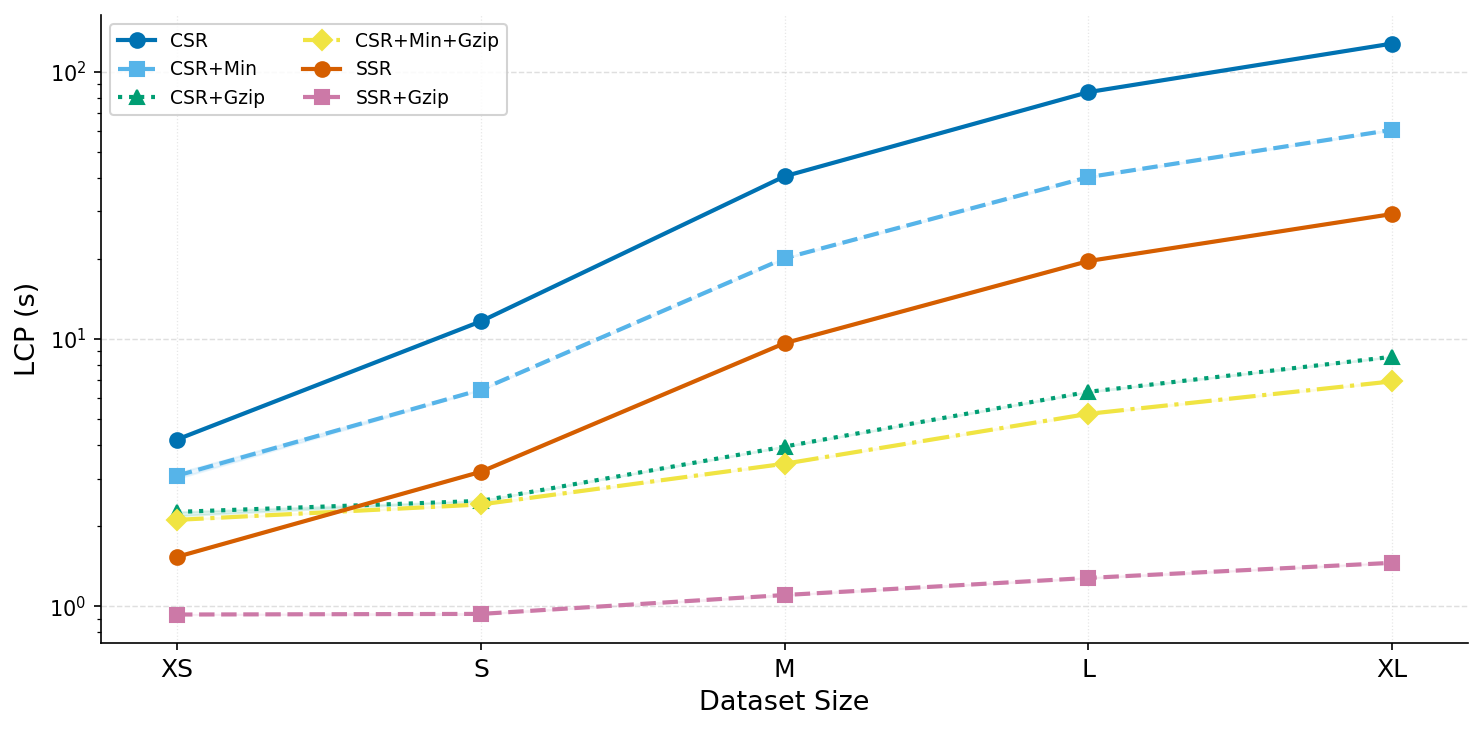
\includegraphics[width=\textwidth, keepaspectratio]{img/lcp.png}
    \caption{LCP values}
    \label{fig:lcp}
\end{figure*}

\paragraph{\textbf{First Contentful Paint}}
The FCP metric refers to the time between when the user navigates to the page and when the first piece of content is rendered on the screen. A good experience occurs when this value is up to 1.8s, while values above 3s are considered poor. Figure~\ref{fig:fcp} presents the boxplot with the results. For smaller datasets, both server-side and client-side rendering provide fast user experiences. As data volume increases, SSR shows a significant increase in loading time, while CSR maintains consistently good performance compared to SSR.

\begin{figure*}[tb]
    \centering
    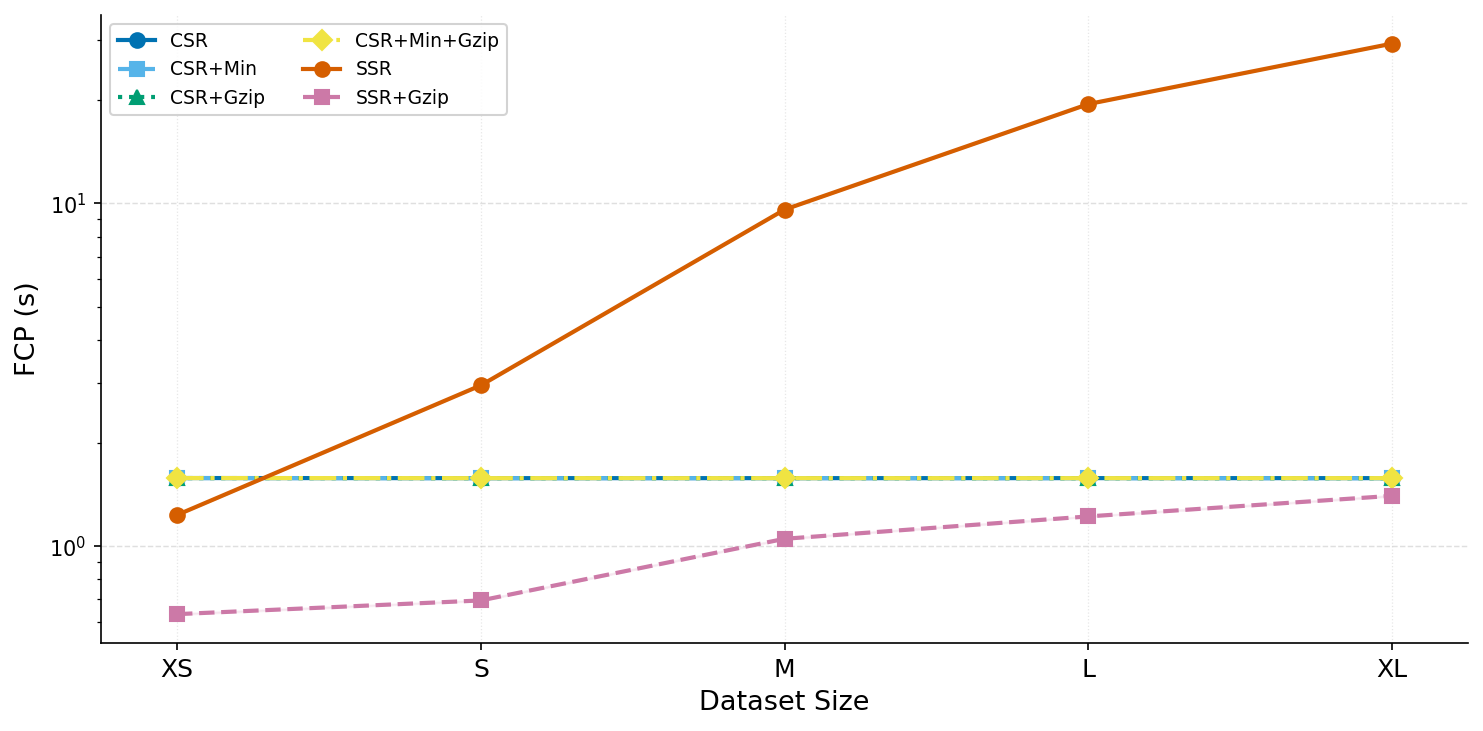
\includegraphics[width=\textwidth, keepaspectratio]{img/fcp.png}
    \caption{FCP values}
    \label{fig:fcp}
\end{figure*}



\paragraph{\textbf{Speed Index}}
The SI metric measures the speed at which content is displayed during page loading. Lighthouse classifies times up to 3.4s as fast, between 3.4s and 5.8s as moderate, and above 5.8s as slow. Figure~\ref{fig:si} shows the boxplot with the results. For smaller data sizes, SI followed the same trend as the LCP and FCP metrics, with both rendering methods showing comparable loading times. However, with larger data volumes, there was a significant performance degradation in server-side rendering, resulting in worse outcomes.

\begin{figure*}[h]
    \centering
    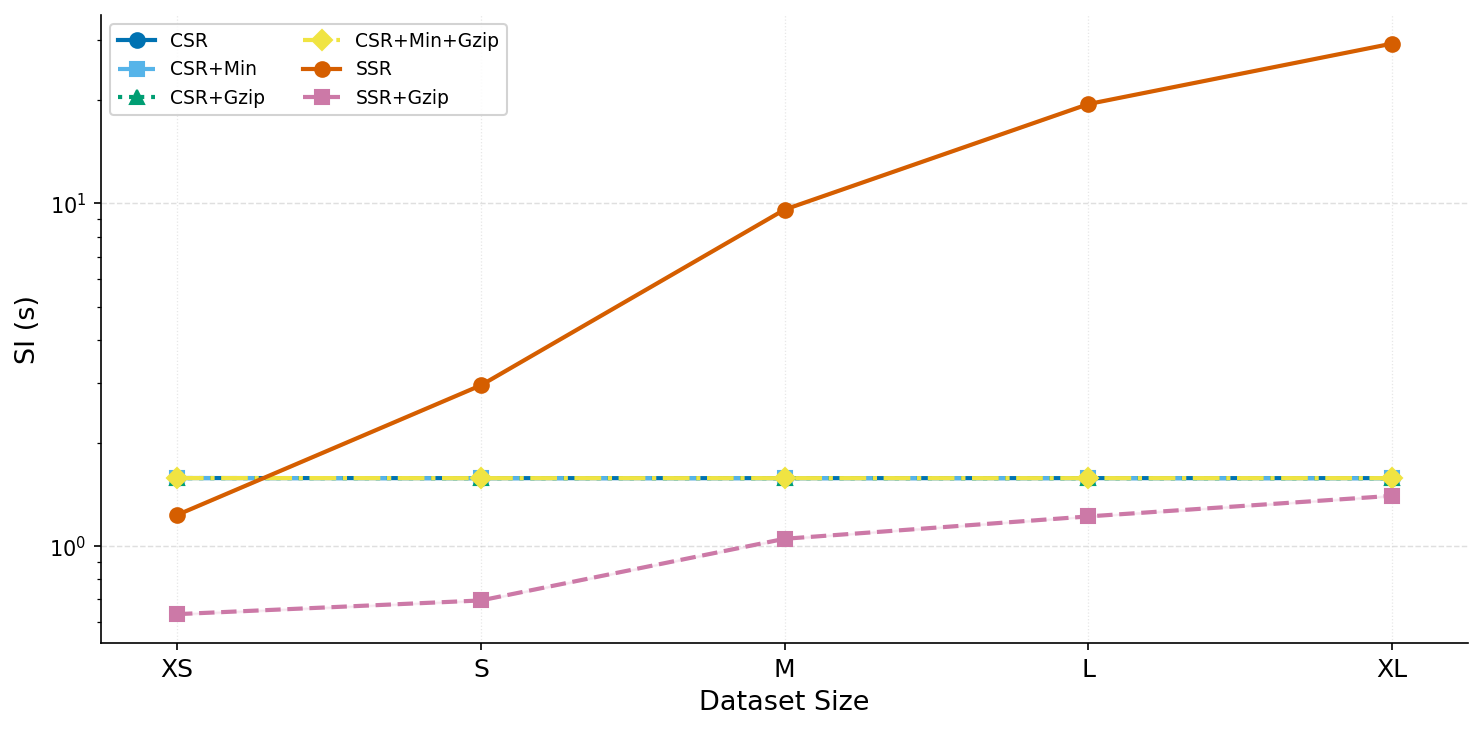
\includegraphics[width=\textwidth, keepaspectratio]{img/si.png}
    \caption{SI values}
    \label{fig:si}
\end{figure*}

\paragraph{\textbf{Time to Interactive}}
The TTI metric measures how long it takes for the page to become fully interactive. Lighthouse considers times up to 3.4s as fast, between 3.4s and 5.8s as moderate, and above 5.8s as slow. Figure~\ref{fig:tti} shows the boxplot with the results. SSR showed shorter loading times compared to CSR across all data sizes.

\begin{figure*}[h]
    \centering
    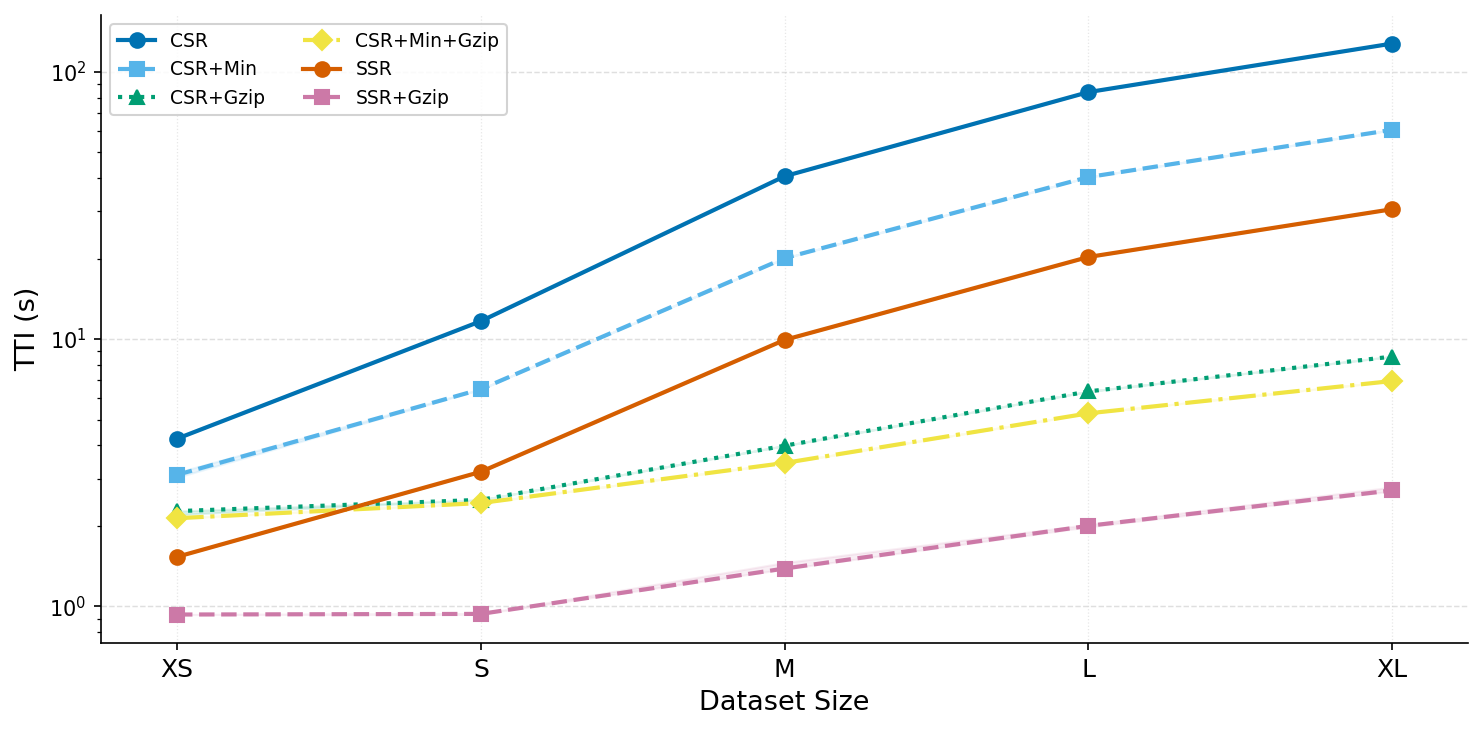
\includegraphics[width=\textwidth, keepaspectratio]{img/tti.png}
    \caption{TTI values}
    \label{fig:tti}
\end{figure*}

\paragraph{\textbf{JS Heap Size}}
The \textit{JS Heap Size} metric refers to the memory space allocated for storing JavaScript objects. Although there is no standardized quality threshold, it was observed that CSR and SSR had similar memory usage for smaller data sizes. However, memory consumption increased significantly for CSR with larger datasets. Figure~\ref{fig:jsheap} shows the boxplot with the results.

\begin{figure*}[h]
    \centering
    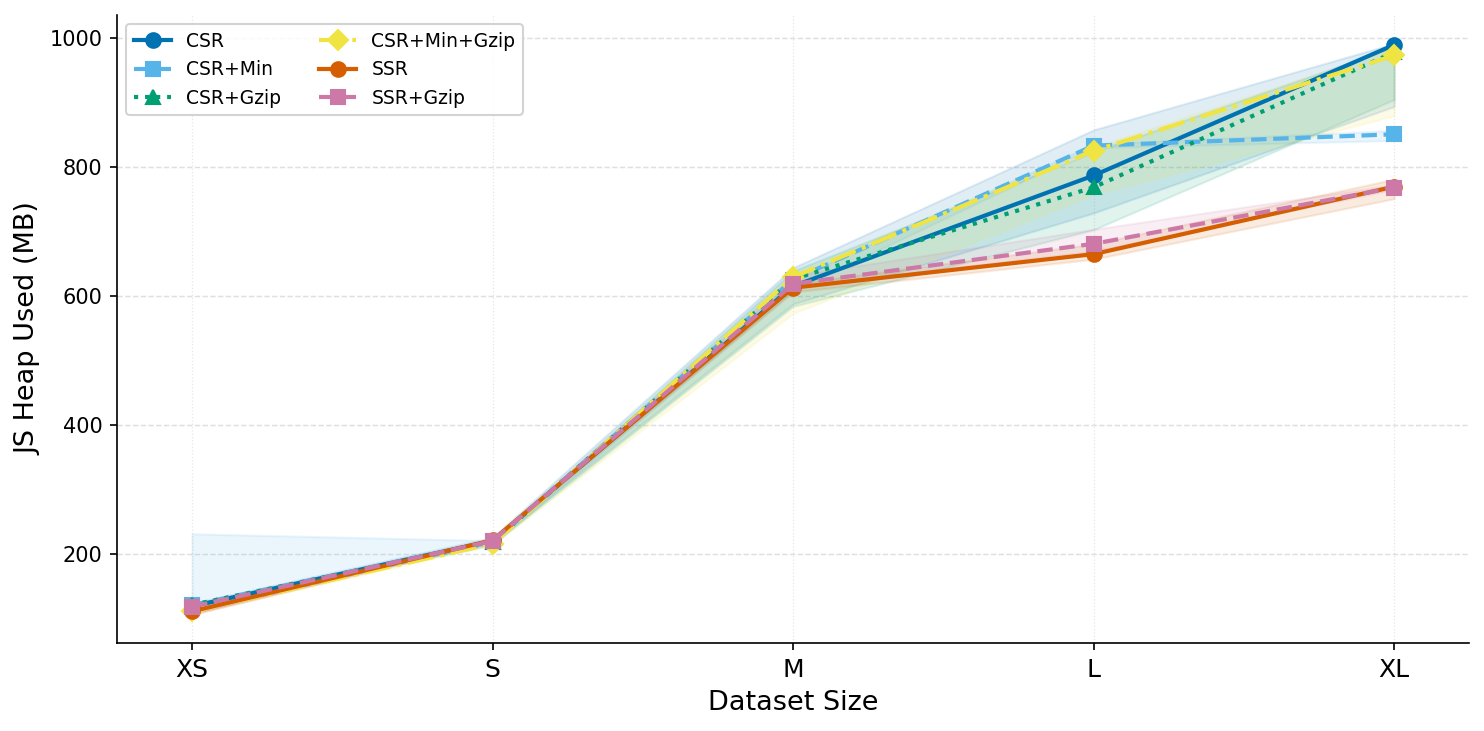
\includegraphics[width=\textwidth, keepaspectratio]{img/jsheap.png}
    \caption{\textit{JS Heap} memory usage}
    \label{fig:jsheap}
\end{figure*}

\subsection{Statistical Analysis}
All results discussed in the previous sections were considered for the statistical analysis. The Shapiro-Wilk test was performed to assess data normality. Next, non-parametric variance analyses (Kruskal-Wallis) were conducted to compare the results. A $p$-value below 0.05 was considered statistically significant, indicating a 95\% confidence level.

Table~\ref{tabela:estatistica} presents the results of the statistical tests for each metric, highlighting the impact of the rendering method factor on the analyzed metrics. These results suggest statistically significant differences ($p$-value $\leq$ 0.05) across all variables based on the rendering method factor.

\begin{table*}[!t]
\centering
\footnotesize
\caption{Kruskal-Wallis test results per metric and dataset size (CSR vs.\ SSR baseline)}
\label{tabela:estatistica}
\begin{tabular}{|l|c|c|c|c|c|c|c|c|c|c|}
\hline
\multirow{2}{*}{\textbf{Metric}} &
\multicolumn{2}{c|}{\textbf{Extra-Small}} &
\multicolumn{2}{c|}{\textbf{Small}} &
\multicolumn{2}{c|}{\textbf{Medium}} &
\multicolumn{2}{c|}{\textbf{Large}} &
\multicolumn{2}{c|}{\textbf{Extra-Large}} \\
\cline{2-11}
& \textbf{H} & \textbf{\textit{p}} & \textbf{H} & \textbf{\textit{p}} & \textbf{H} & \textbf{\textit{p}} & \textbf{H} & \textbf{\textit{p}} & \textbf{H} & \textbf{\textit{p}} \\
\hline
LCP      & 14.29 & $1.57{\times}10^{-4}$ & 14.29 & $1.57{\times}10^{-4}$ & 14.29 & $1.57{\times}10^{-4}$ & 14.29 & $1.57{\times}10^{-4}$ & 14.29 & $1.57{\times}10^{-4}$ \\
FCP      & 14.29 & $1.57{\times}10^{-4}$ & 14.29 & $1.57{\times}10^{-4}$ & 14.29 & $1.57{\times}10^{-4}$ & 14.30 & $1.56{\times}10^{-4}$ & 14.29 & $1.57{\times}10^{-4}$ \\
SI       & 14.29 & $1.57{\times}10^{-4}$ & 14.29 & $1.57{\times}10^{-4}$ & 14.29 & $1.57{\times}10^{-4}$ & 14.30 & $1.56{\times}10^{-4}$ & 14.29 & $1.57{\times}10^{-4}$ \\
TTI      & 14.29 & $1.57{\times}10^{-4}$ & 14.29 & $1.57{\times}10^{-4}$ & 14.29 & $1.57{\times}10^{-4}$ & 14.29 & $1.57{\times}10^{-4}$ & 14.29 & $1.57{\times}10^{-4}$ \\
JS Heap  &  2.52 & $1.12{\times}10^{-1}$ &  0.37 & $5.45{\times}10^{-1}$ &  0.01 & $9.40{\times}10^{-1}$ & 14.29 & $1.57{\times}10^{-4}$ & 13.72 & $2.12{\times}10^{-4}$ \\
\hline
\end{tabular}
\vspace{2pt}
\begin{flushleft}
\footnotesize
Significance level: $\alpha = 0.05$. Bold $p$-values indicate no significant difference.
\end{flushleft}
\end{table*}



\subsection{\texorpdfstring{\textcolor{darkgreen}{Resultados com Técnicas de Otimização}}{Resultados com Técnicas de Otimização}}
\label{sec:optimization_results}

\textcolor{darkgreen}{Para avaliar o impacto das técnicas de otimização descritas na Seção~\ref{sec:optimization_techniques}, o experimento foi ampliado para incluir seis condições experimentais: CSR sem otimização (\textit{baseline}), CSR com minificação, CSR com compressão gzip, CSR com minificação e gzip combinados, SSR sem otimização (\textit{baseline}) e SSR com compressão gzip. A Tabela~\ref{tab:extended_medians} apresenta os valores medianos das métricas LCP, FCP, TTI e \textit{JS Heap} para cada condição e tamanho de dados. A minificação não foi aplicada à SSR, uma vez que o conteúdo HTML gerado pelo servidor já é entregue em formato compacto, sem redundâncias estruturais equivalentes às presentes nos dados JSON brutos.}

\begin{table*}[!t]
\centering
\footnotesize
\caption{\textcolor{darkgreen}{Medianas de LCP, FCP, TTI (s) e JS Heap (MB) por condição e tamanho de conjunto de dados}}
\label{tab:extended_medians}
\begin{tabular}{|l|l|c|c|c|c|c|}
\hline
\textbf{Métrica} & \textbf{Condição} & \textbf{XS} & \textbf{S} & \textbf{M} & \textbf{L} & \textbf{XL} \\
\hline
\multirow{6}{*}{\textbf{LCP (s)}}
  & CSR                       & 4,21  & 11,64 & 40,61 & 83,85  & 127,39 \\ \cline{2-7}
  & CSR + Minificação         & 3,08  &  6,46 & 20,05 & 40,32  &  60,59 \\ \cline{2-7}
  & CSR + Gzip                & 2,26  &  2,48 &  3,96 &  6,35  &   8,58 \\ \cline{2-7}
  & CSR + Min.\ + Gzip        & 2,11  &  2,41 &  3,42 &  5,25  &   6,95 \\ \cline{2-7}
  & SSR                       & 1,53  &  3,19 &  9,65 & 19,57  &  29,34 \\ \cline{2-7}
  & \textbf{SSR + Gzip}       & \textbf{0,93} & \textbf{0,94} & \textbf{1,10} & \textbf{1,28} & \textbf{1,46} \\
\hline
\multirow{6}{*}{\textbf{FCP (s)}}
  & CSR                       & 1,58  & 1,58  & 1,58  &  1,58  &  1,58 \\ \cline{2-7}
  & CSR + Minificação         & 1,58  & 1,58  & 1,58  &  1,58  &  1,58 \\ \cline{2-7}
  & CSR + Gzip                & 1,58  & 1,58  & 1,58  &  1,58  &  1,58 \\ \cline{2-7}
  & CSR + Min.\ + Gzip        & 1,58  & 1,58  & 1,58  &  1,58  &  1,58 \\ \cline{2-7}
  & SSR                       & 1,23  & 2,95  & 9,60  & 19,51  & 29,28 \\ \cline{2-7}
  & \textbf{SSR + Gzip}       & \textbf{0,63} & \textbf{0,69} & \textbf{1,05} & \textbf{1,22} & \textbf{1,40} \\
\hline
\multirow{6}{*}{\textbf{TTI (s)}}
  & CSR                       & 4,24  & 11,66 & 40,64 & 83,87  & 127,41 \\ \cline{2-7}
  & CSR + Minificação         & 3,10  &  6,49 & 20,08 & 40,35  &  60,62 \\ \cline{2-7}
  & CSR + Gzip                & 2,27  &  2,50 &  3,99 &  6,37  &   8,60 \\ \cline{2-7}
  & CSR + Min.\ + Gzip        & 2,14  &  2,44 &  3,44 &  5,27  &   6,97 \\ \cline{2-7}
  & SSR                       & 1,53  &  3,19 &  9,93 & 20,27  &  30,60 \\ \cline{2-7}
  & \textbf{SSR + Gzip}       & \textbf{0,93} & \textbf{0,94} & \textbf{1,39} & \textbf{2,00} & \textbf{2,72} \\
\hline
\multirow{6}{*}{\textbf{JS Heap (MB)}}
  & CSR                       & 119,49 & 220,72 & 615,12 & 786,58 & 988,90 \\ \cline{2-7}
  & CSR + Minificação         & 121,42 & 219,59 & 625,39 & 832,83 & 850,38 \\ \cline{2-7}
  & CSR + Gzip                & 121,46 & 218,63 & 626,12 & 768,27 & 977,44 \\ \cline{2-7}
  & CSR + Min.\ + Gzip        & \textbf{111,55} & \textbf{216,38} & 629,11 & 824,76 & 972,55 \\ \cline{2-7}
  & SSR                       & 111,67 & 221,74 & \textbf{612,79} & \textbf{664,81} & 769,32 \\ \cline{2-7}
  & SSR + Gzip                & 118,99 & 220,46 & 618,69 & 680,80 & \textbf{767,71} \\
\hline
\end{tabular}
\vspace{2pt}
\begin{flushleft}
\footnotesize
\textbf{*} Em negrito: melhor resultado por métrica e tamanho (menor é melhor).
XS = Extra-Small ($\approx$498~kB); S = Small ($\approx$2~MB); M = Medium ($\approx$7,9~MB); L = Large ($\approx$16,8~MB); XL = Extra-Large ($\approx$26~MB).
\end{flushleft}
\end{table*}


\textcolor{darkgreen}{Os resultados indicam que a compressão gzip foi a otimização com maior impacto sobre as métricas LCP e TTI na abordagem CSR. No tamanho XL, o LCP mediano reduziu de 127{,}39s (CSR \textit{baseline}) para 8{,}58s com gzip (redução de 93{,}3\%) e para 6{,}95s com a combinação de minificação e gzip (redução de 94{,}5\%). A minificação isolada também se mostrou relevante, reduzindo o LCP de 127{,}39s para 60{,}59s (redução de 52{,}4\%). Para a SSR, a aplicação de gzip reduziu o LCP mediano de 29{,}35s para 1{,}46s no tamanho XL (redução de 95{,}0\%).}

\textcolor{darkgreen}{Para a métrica FCP, as otimizações aplicadas à CSR não produziram alterações perceptíveis: todas as variantes CSR mantiveram FCP estável em torno de 1{,}58s, independentemente do tamanho dos dados. Esse comportamento é esperado, uma vez que a CSR renderiza a estrutura inicial da página antes de carregar os dados via JavaScript. Na SSR, por outro lado, o FCP é diretamente afetado pelo volume de dados, pois o navegador precisa receber todo o HTML antes de iniciar a renderização. Sem gzip, o FCP da SSR alcançou 29{,}28s no tamanho XL, enquanto com gzip foi reduzido para 1{,}40s.}

\textcolor{darkgreen}{O consumo de memória (\textit{JS Heap}) apresentou diferenças relevantes apenas nos tamanhos Large e Extra Large. Para dados menores, os valores foram comparáveis entre todas as condições. No tamanho XL, as variantes CSR consumiram entre 851 e 989~MB, enquanto ambas as variantes SSR ficaram em torno de 770~MB, indicando que a SSR utiliza menos memória JavaScript para processar grandes volumes de dados.}

\textcolor{darkgreen}{A Tabela~\ref{tab:kruskal-ext} apresenta os resultados do teste de Kruskal-Wallis para o experimento ampliado, considerando os seis grupos experimentais. Diferenças estatisticamente significativas ($p < 0{,}05$) foram observadas para LCP, FCP, SI e TTI em todos os tamanhos de dados. Para o \textit{JS Heap}, o teste não identificou diferenças significativas nos tamanhos XS ($p = 0{,}055$), S ($p = 0{,}063$) e M ($p = 0{,}919$), corroborando a observação de que o consumo de memória se torna um fator diferenciador apenas em grandes volumes de dados.}

\begin{table}[!ht]
\centering
\footnotesize
\caption{\textcolor{darkgreen}{Resultados do teste de Kruskal-Wallis por métrica e tamanho (experimento estendido, 6~condições)}}
\label{tab:kruskal-ext}
\begin{tabular}{|c|l|c|c|}
\hline
\textbf{Tamanho} & \textbf{Métrica} & \textbf{Estatística H} & \textbf{\textit{p}-valor} \\
\hline
\multirow{5}{*}{\textbf{XS}}
  & LCP       & 56,45 & $6{,}56{\times}10^{-11}$ \\ \cline{2-4}
  & FCP       & 57,38 & $4{,}23{\times}10^{-11}$ \\ \cline{2-4}
  & SI        & 57,38 & $4{,}23{\times}10^{-11}$ \\ \cline{2-4}
  & TTI       & 56,45 & $6{,}56{\times}10^{-11}$ \\ \cline{2-4}
  & Score     & 32,25 & $5{,}29{\times}10^{-6}$  \\ \hline
\multirow{5}{*}{\textbf{S}}
  & LCP       & 57,38 & $4{,}23{\times}10^{-11}$ \\ \cline{2-4}
  & FCP       & 57,38 & $4{,}23{\times}10^{-11}$ \\ \cline{2-4}
  & SI        & 57,38 & $4{,}23{\times}10^{-11}$ \\ \cline{2-4}
  & TTI       & 57,38 & $4{,}23{\times}10^{-11}$ \\ \cline{2-4}
  & Score     & 58,49 & $2{,}49{\times}10^{-11}$ \\ \hline
\multirow{5}{*}{\textbf{M}}
  & LCP       & 57,38 & $4{,}23{\times}10^{-11}$ \\ \cline{2-4}
  & FCP       & 57,38 & $4{,}23{\times}10^{-11}$ \\ \cline{2-4}
  & SI        & 57,38 & $4{,}23{\times}10^{-11}$ \\ \cline{2-4}
  & TTI       & 57,38 & $4{,}23{\times}10^{-11}$ \\ \cline{2-4}
  & Score     & 53,59 & $2{,}55{\times}10^{-10}$ \\ \hline
\multirow{5}{*}{\textbf{L}}
  & LCP       & 57,38 & $4{,}23{\times}10^{-11}$ \\ \cline{2-4}
  & FCP       & 57,38 & $4{,}23{\times}10^{-11}$ \\ \cline{2-4}
  & SI        & 57,38 & $4{,}23{\times}10^{-11}$ \\ \cline{2-4}
  & TTI       & 57,38 & $4{,}23{\times}10^{-11}$ \\ \cline{2-4}
  & Score     & 56,43 & $6{,}61{\times}10^{-11}$ \\ \hline
\multirow{5}{*}{\textbf{XL}}
  & LCP       & 57,38 & $4{,}23{\times}10^{-11}$ \\ \cline{2-4}
  & FCP       & 57,38 & $4{,}23{\times}10^{-11}$ \\ \cline{2-4}
  & SI        & 57,38 & $4{,}23{\times}10^{-11}$ \\ \cline{2-4}
  & TTI       & 57,38 & $4{,}23{\times}10^{-11}$ \\ \cline{2-4}
  & Score     & 54,01 & $2{,}09{\times}10^{-10}$ \\ \hline
\end{tabular}
\end{table}


\textcolor{darkgreen}{A Tabela~\ref{tab:cliffs-delta} apresenta os valores de Cliff's Delta para as comparações mais relevantes: o efeito das otimizações sobre cada abordagem (CSR \textit{baseline} vs. CSR com minificação e gzip; SSR \textit{baseline} vs. SSR com gzip) e a comparação entre as melhores configurações de cada abordagem (CSR com minificação e gzip vs. SSR com gzip). Para LCP e TTI, todas as comparações apresentaram tamanhos de efeito grandes ($|\delta| = 1{,}0$) em todos os tamanhos de dados, indicando separação completa entre as distribuições. Para FCP, as otimizações não alteraram o comportamento da CSR (efeitos negligenciáveis entre variantes CSR), enquanto a compressão gzip produziu efeito grande na SSR ($\delta = 1{,}0$). Para o \textit{JS Heap}, os efeitos foram negligenciáveis a pequenos nos tamanhos menores, tornando-se grandes apenas nos tamanhos L e XL.}

\begin{table*}[!ht]
\centering
\footnotesize
\caption{\textcolor{darkgreen}{Delta de Cliff ($\delta$) para LCP — comparações par a par selecionadas por tamanho de conjunto de dados}}
\label{tab:cliffs-delta}
\begin{tabular}{|l|c|c|c|c|c|c|}
\hline
\textbf{Comparação} & \textbf{XS} & \textbf{S} & \textbf{M} & \textbf{L} & \textbf{XL} & \textbf{Interpretação} \\
\hline
CSR vs.\ CSR + Gzip               & 1,00 & 1,00 & 1,00 & 1,00 & 1,00 & Grande \\
CSR vs.\ CSR + Minificação        & 1,00 & 1,00 & 1,00 & 1,00 & 1,00 & Grande \\
CSR + Gzip vs.\ CSR + Min.\ + Gzip & 0,66 & 1,00 & 1,00 & 1,00 & 1,00 & Grande \\
CSR + Min.\ + Gzip vs.\ SSR + Gzip & 1,00 & 1,00 & 1,00 & 1,00 & 1,00 & Grande \\
SSR vs.\ SSR + Gzip               & 1,00 & 1,00 & 1,00 & 1,00 & 1,00 & Grande \\
\hline
\end{tabular}
\vspace{2pt}
\begin{flushleft}
\footnotesize
XS = Extra-Small; S = Small; M = Medium; L = Large; XL = Extra-Large.
$\delta = 1{,}0$ com IC$_{95\%}$ $[1{,}0;\,1{,}0]$ indica separação completa entre grupos.
Escala: $|\delta| < 0{,}147$ = negligível; $0{,}147$--$0{,}330$ = pequeno; $0{,}330$--$0{,}474$ = médio; $|\delta| \geq 0{,}474$ = grande~\cite{Romano2006}.
IC de 95\% calculados via \textit{bootstrap}~\cite{efron:1994}.
\end{flushleft}
\end{table*}


\textcolor{darkgreen}{Os resultados da análise de tamanho de efeito permitem verificar as hipóteses formuladas na Seção~\ref{sec:optimization_techniques}. Em relação à \textbf{H1}, a minificação reduziu o LCP mediano da CSR em até 52{,}4\% (tamanho XL), com efeito grande ($\delta = 1{,}0$) em LCP e TTI. Contudo, os efeitos sobre FCP foram negligenciáveis a pequenos, indicando que a minificação impacta o tempo total de carregamento, mas não a renderização inicial da CSR. Em relação à \textbf{H2}, a compressão gzip produziu reduções expressivas em todas as métricas temporais, com efeito grande tanto na CSR (redução de 93{,}3\% no LCP) quanto na SSR (redução de 95{,}0\% no LCP para o tamanho XL). A \textbf{H3} foi parcialmente confirmada: a combinação de minificação e gzip na CSR proporcionou redução de 94{,}5\% no LCP em relação ao \textit{baseline}, superior à minificação isolada (52{,}4\%) e ligeiramente superior à compressão isolada (93{,}3\%), embora o ganho incremental da minificação sobre a compressão gzip tenha sido modesto.}


\section{Discussion}
\label{sec:discussion}
% This section discusses the results of the data collected during the tests and the threats to the validity of this study.

% After data collection, it was possible to observe significant differences across the analyzed metrics. The results show that both rendering strategies performed well with smaller datasets. However, as the data size increased, application performance degraded. SSR achieved better results in the TTI and LCP metrics, while CSR yielded better outcomes in SI and FCP. Regarding JS Heap memory usage, there were no statistically significant differences, as shown in Table~\ref{tabela:estatistica}.

While both rendering strategies demonstrated good performance with smaller datasets, significant differences emerged as data volume increased, directly impacting application efficiency. Specifically, SSR consistently yielded better results for LCP and TTI , likely due to the server delivering a fully rendered HTML page, allowing the browser to display core content and become interactive more rapidly without extensive client-side JavaScript processing. Conversely, CSR exhibited superior performance in FCP and SI, especially with larger datasets where its ability to dynamically render content once initial scripts are loaded minimized the time to render visible elements. This distinction suggests that for content-heavy applications where initial load and SEO are paramount, SSR may be more advantageous, whereas highly interactive applications might benefit from CSR's dynamic rendering capabilities after initial asset loading. Regarding \textit{JS Heap} memory usage, there were no statistically significant differences, as shown in Table~\ref{tabela:estatistica}.

This study supports the findings of \citet{meredova2023ssr}, which analyzed server-side rendering (SSR) capabilities using the React and Vue front-end libraries. According to the study, the SSR approach enhances the user experience by reducing the initial page load time. This advantage makes SSR suitable for devices with slower internet connections and for applications where fast content loading is essential.

\textcolor{darkgreen}{A análise por meio do Cliff's Delta complementa os resultados dos testes de significância ao revelar a magnitude prática das diferenças. Conforme apresentado na Tabela~\ref{tab:cliffs-delta}, para LCP e TTI os tamanhos de efeito foram consistentemente grandes ($|\delta| = 1{,}0$) em todas as comparações e tamanhos de dados, confirmando que as diferenças de desempenho entre as abordagens de renderização e entre as configurações com e sem otimização são não apenas estatisticamente significativas, mas também relevantes do ponto de vista prático. Para a métrica \textit{JS Heap}, entretanto, apesar de $p$-values significativos nos tamanhos L e XL (Tabela~\ref{tab:kruskal-ext}), os valores de Cliff's Delta entre variantes da mesma abordagem indicaram efeitos pequenos a médios. Essa discrepância entre significância estatística e tamanho de efeito ilustra um cenário em que o $p$-value isoladamente superestimaria a diferença prática no consumo de memória, reforçando a importância de se reportar medidas de tamanho de efeito em estudos empíricos de engenharia de software \cite{Kitchenham2024, Kitchenham2017}.}

\textcolor{darkgreen}{Os resultados com otimizações evidenciam que a compressão gzip é o fator de maior impacto sobre o desempenho de ambas as abordagens, sendo capaz de reduzir o LCP em mais de 90\% nos maiores volumes de dados. Esse achado é consistente com os resultados de \citet{jsonXmlApiResponse:2021} e \citet{dataConsumptionIot:2021}, que demonstraram a eficácia da compressão na redução do volume de dados trafegados. Quando combinadas as melhores configurações de cada abordagem (CSR com minificação e gzip vs. SSR com gzip), a SSR manteve desempenho superior em LCP e TTI, com efeito grande em todos os tamanhos. Contudo, a CSR otimizada apresentou valores absolutos substancialmente menores do que a CSR \textit{baseline}, o que indica que, em cenários nos quais a adoção de SSR não é viável, a combinação de minificação e compressão pode reduzir consideravelmente a desvantagem da CSR em relação à SSR.}

\section{Threats to Validity}\label{sec:threats_to_validity}

This section addresses the potential threats to validity across different dimensions and the strategies adopted to mitigate them \cite{book:wohlin}.

\textbf{Internal Validity.}
For internal validity, factors such as hardware and software influence on the stability of the results were considered. To mitigate these interferences, all tests were executed in a local environment, on the same machine and operating system. Additionally, each experiment was run ten times, ensuring that the observed results are consistent and not merely due to random chance or transient system variations. This repetition enhances the reliability of the findings by providing more robust and representative data averages.

\textcolor{darkgreen}{Nesta versão estendida, a minificação foi aplicada apenas ao JSON da CSR, sem contrapartida nas respostas HTML da SSR. A minificação de HTML envolve mecanismo diferente e está fora do escopo deste trabalho, mas a assimetria limita comparações diretas entre os efeitos de minificação nas duas estratégias. As conclusões sobre minificação valem, portanto, para arquiteturas CSR. A sobrecarga de CPU imposta pelo gzip no servidor também não foi medida, o que pode limitar a generalização dos ganhos de latência em ambientes com processamento restrito.}

\textbf{External Validity.}
Regarding external validity, a recognized limitation of this study is that the experiments were conducted within a single execution environment. All experiments were executed on a single hardware configuration (a MacBook Air M2) and within a single browser environment (Chromium). This restricted setup constrains the generalizability of the findings, as performance and behavior may vary across distinct hardware platforms, operating systems, and browsers employing different rendering engines. However, with the environment used, relevant insights were found for the study proposal, which can be expanded in future work.

\textcolor{darkgreen}{Os experimentos foram conduzidos em \textit{localhost}, sem latência de rede ou limitação de largura de banda, o que provavelmente subestima o benefício do gzip em implantações reais. \citet{ollila:2021} verificou que diferenças de desempenho entre estratégias de renderização variam conforme o motor JavaScript, sugerindo que as magnitudes aqui reportadas podem não se reproduzir com outros frameworks. O domínio avaliado, uma galeria de fotos com metadados de imagens, representa uma aplicação de conteúdo estático; a generalização para SPAs interativas, \textit{dashboards} ou e-commerce é limitada \cite{gangishetti:2026}.}

\textbf{Conclusion Validity.}

With respect to conclusion validity, several techniques exist to improve application performance, such as data minification and compression, asynchronous loading (lazy loading), the use of Content Delivery Networks (CDNs), image preloading, and data caching. \textcolor{darkgreen}{Esta versão estendida investiga diretamente duas dessas técnicas, minificação e gzip, em um experimento fatorial controlado, endereçando uma limitação do estudo original.} \todo{However, the objective of this study was to analyze the impact of the rendering approach (SSR and CSR) and data size on the user experience.} To ensure that the evaluation focus remained on rendering performance, the application used only HTML, CSS, and JavaScript without any external libraries.

\textcolor{darkgreen}{A análise estendida utiliza o teste \textit{post-hoc} de Dunn com correção de Holm para controlar o erro familiar nas comparações múltiplas \cite{book:wohlin} e o Delta de Cliff com intervalos de confiança via \textit{bootstrap} para estimar o tamanho de efeito \cite{efron:1994,Kitchenham2024}. Com $n = 10$ observações por célula, o poder estatístico é suficiente apenas para detectar efeitos grandes ($|\delta| \geq 0{,}474$); as conclusões ficam restritas a esse nível.}

\textbf{\textcolor{darkgreen}{Construct Validity.}}
\textcolor{darkgreen}{As métricas \textit{Core Web Vitals} (LCP, FCP, SI, TTI, CLS, FID e Lighthouse Score) têm correlação documentada com comportamento do usuário, incluindo taxa de rejeição e conversão \cite{sikder:2016}. O Lighthouse Score, por ser composto, pode não capturar todas as dimensões da experiência percebida em aplicações com interação complexa. O mapeamento de \texttt{format=html} para SSR e \texttt{format=json} para CSR é uma simplificação dos paradigmas; \textit{frameworks} modernos como Next.js, Nuxt, React e Svelte podem apresentar características distintas \cite{ollila:2021}. Os resultados caracterizam os \textit{trade-offs} entre HTML pré-renderizado e renderização de JSON no cliente, não o desempenho de \textit{frameworks} de produção.}



\section{Conclusion}\label{sec:conclusion}

This study compared the performance between two types of rendering in web applications, using Google's Core Web Vitals metrics as a quality assessment approach. For the analysis, both CSR and SSR rendering strategies were evaluated. A photo gallery application was developed for each rendering approach, and aspects such as performance, user experience, and memory usage were compared.

For data collection, a Node.js script was created using the Lighthouse performance measurement tool. The Kruskal-Wallis statistical test was applied to compare the results and verify the presence of statistically significant differences. The tests indicated relevant differences. \todo{One hypothesis raised is that CSR rendering provides better performance in metrics related to the loading of visible content, such as FCP and SI, while SSR rendering presents better results in metrics related to interactivity and loading of the largest page content, such as TTI and LCP. The results suggest that the choice between CSR and SSR should consider the specific objectives of the application and its usage environment.}

\textcolor{darkgreen}{A versão estendida amplia o design original com dois fatores adicionais: minificação de JSON e compressão HTTP via gzip. O experimento abrangeu 30 condições de tratamento e 300 observações, cobrindo as cinco faixas de tamanho de dados em todas as configurações avaliadas.}

\textcolor{darkgreen}{A compressão gzip foi a otimização de maior impacto: reduziu o LCP mediano do CSR em 93{,}3\% no tamanho Extra-Large (de 127{,}39~s para 8{,}58~s) e o da SSR em 95{,}0\% (de 29{,}35~s para 1{,}46~s). A minificação do JSON também reduziu o LCP da CSR de forma relevante, em torno de 51--52\% nos tamanhos médio a grande sem compressão, mas o ganho incremental ao combiná-la com gzip foi modesto (cerca de 19\% no Extra-Large). O SSR com gzip superou todas as variantes CSR em LCP e TTI com margem crescente conforme o payload aumenta: 2{,}3$\times$ mais rápido que o CSR com minificação e gzip no Extra-Small e 4{,}8$\times$ no Extra-Large. Os tamanhos de efeito confirmam essa separação, com $\delta = 1{,}0$ em todas as comparações entre SSR + Gzip e configurações CSR \cite{Cliff1993,Romano2006}.}

\textcolor{darkgreen}{O FCP no CSR permaneceu em torno de 1{,}58~s independentemente do uso de gzip ou minificação, indicando que essa métrica reflete o carregamento do \textit{script} inicial e não é sensível a otimizações de transferência de dados. Para avaliar o impacto dessas técnicas, LCP e TTI são as métricas adequadas, conforme \citet{verma:2024}.}

\textcolor{darkgreen}{A compressão gzip deve ser habilitada em qualquer aplicação que utilize SSR ou CSR, dado o impacto expressivo com custo de implementação baixo \cite{sikder:2016}. A minificação de JSON é útil como técnica complementar na CSR, em especial quando o gzip não está disponível. Quando LCP e TTI são as métricas prioritárias, como em plataformas de conteúdo com volumes maiores de dados \cite{gangishetti:2026}, o SSR com gzip oferece vantagem consistente sobre qualquer configuração CSR. Em aplicações com \textit{payloads} pequenos onde o FCP é crítico, o CSR otimizado mantém desempenho competitivo.}

As future work, we suggest \textcolor{darkgreen}{avaliar o efeito da minificação de HTML sobre o desempenho do SSR, ainda não investigado, de forma a comparar os efeitos de minificação nas duas estratégias de forma simétrica. Recomenda-se também} analyzing other rendering approaches in web applications, such as Incremental Static Regeneration (ISR) and isomorphic architecture. \todo{It is also recommended to perform tests on mobile devices and under varying bandwidth conditions, given the relevance of such access scenarios to ensure an optimized and consistent experience across different platforms and contexts.} \textcolor{darkgreen}{Testes com \textit{throttling} de rede (3G e 4G) esclareceriam se a vantagem do gzip aumenta ainda mais em conexões lentas. Medir o custo de CPU do gzip no servidor sob alta concorrência completaria a análise de custo-benefício. Replicar o estudo com \textit{frameworks} de produção como Next.js, Nuxt, SvelteKit e React em múltiplos navegadores endereçaria a limitação de validade de construto da Seção~\ref{sec:threats_to_validity} \cite{ollila:2021}.} Additionally, future research should include a broader range of application types, such as e-commerce platforms, dashboards, and complex single-page applications, to strengthen the generalizability of the findings.


\section*{ARTIFACT AVAILABILITY}
The \textit{scripts} and \textit{dataset} are available at:
\url{https://github.com/CleitonSilvaT/cs-vs-ssr-sbqs-2025}

\bibliographystyle{apalike}
\bibliography{sample-base}

\end{document}
